% Options for packages loaded elsewhere
\PassOptionsToPackage{unicode}{hyperref}
\PassOptionsToPackage{hyphens}{url}
\PassOptionsToPackage{dvipsnames,svgnames,x11names}{xcolor}
%
\documentclass[
  letterpaper,
  DIV=11,
  numbers=noendperiod]{scrartcl}

\usepackage{amsmath,amssymb}
\usepackage{iftex}
\ifPDFTeX
  \usepackage[T1]{fontenc}
  \usepackage[utf8]{inputenc}
  \usepackage{textcomp} % provide euro and other symbols
\else % if luatex or xetex
  \usepackage{unicode-math}
  \defaultfontfeatures{Scale=MatchLowercase}
  \defaultfontfeatures[\rmfamily]{Ligatures=TeX,Scale=1}
\fi
\usepackage{lmodern}
\ifPDFTeX\else  
    % xetex/luatex font selection
\fi
% Use upquote if available, for straight quotes in verbatim environments
\IfFileExists{upquote.sty}{\usepackage{upquote}}{}
\IfFileExists{microtype.sty}{% use microtype if available
  \usepackage[]{microtype}
  \UseMicrotypeSet[protrusion]{basicmath} % disable protrusion for tt fonts
}{}
\makeatletter
\@ifundefined{KOMAClassName}{% if non-KOMA class
  \IfFileExists{parskip.sty}{%
    \usepackage{parskip}
  }{% else
    \setlength{\parindent}{0pt}
    \setlength{\parskip}{6pt plus 2pt minus 1pt}}
}{% if KOMA class
  \KOMAoptions{parskip=half}}
\makeatother
\usepackage{xcolor}
\setlength{\emergencystretch}{3em} % prevent overfull lines
\setcounter{secnumdepth}{-\maxdimen} % remove section numbering
% Make \paragraph and \subparagraph free-standing
\ifx\paragraph\undefined\else
  \let\oldparagraph\paragraph
  \renewcommand{\paragraph}[1]{\oldparagraph{#1}\mbox{}}
\fi
\ifx\subparagraph\undefined\else
  \let\oldsubparagraph\subparagraph
  \renewcommand{\subparagraph}[1]{\oldsubparagraph{#1}\mbox{}}
\fi


\providecommand{\tightlist}{%
  \setlength{\itemsep}{0pt}\setlength{\parskip}{0pt}}\usepackage{longtable,booktabs,array}
\usepackage{calc} % for calculating minipage widths
% Correct order of tables after \paragraph or \subparagraph
\usepackage{etoolbox}
\makeatletter
\patchcmd\longtable{\par}{\if@noskipsec\mbox{}\fi\par}{}{}
\makeatother
% Allow footnotes in longtable head/foot
\IfFileExists{footnotehyper.sty}{\usepackage{footnotehyper}}{\usepackage{footnote}}
\makesavenoteenv{longtable}
\usepackage{graphicx}
\makeatletter
\def\maxwidth{\ifdim\Gin@nat@width>\linewidth\linewidth\else\Gin@nat@width\fi}
\def\maxheight{\ifdim\Gin@nat@height>\textheight\textheight\else\Gin@nat@height\fi}
\makeatother
% Scale images if necessary, so that they will not overflow the page
% margins by default, and it is still possible to overwrite the defaults
% using explicit options in \includegraphics[width, height, ...]{}
\setkeys{Gin}{width=\maxwidth,height=\maxheight,keepaspectratio}
% Set default figure placement to htbp
\makeatletter
\def\fps@figure{htbp}
\makeatother

\KOMAoption{captions}{tableheading}
\makeatletter
\makeatother
\makeatletter
\makeatother
\makeatletter
\@ifpackageloaded{caption}{}{\usepackage{caption}}
\AtBeginDocument{%
\ifdefined\contentsname
  \renewcommand*\contentsname{Table of contents}
\else
  \newcommand\contentsname{Table of contents}
\fi
\ifdefined\listfigurename
  \renewcommand*\listfigurename{List of Figures}
\else
  \newcommand\listfigurename{List of Figures}
\fi
\ifdefined\listtablename
  \renewcommand*\listtablename{List of Tables}
\else
  \newcommand\listtablename{List of Tables}
\fi
\ifdefined\figurename
  \renewcommand*\figurename{Figure}
\else
  \newcommand\figurename{Figure}
\fi
\ifdefined\tablename
  \renewcommand*\tablename{Table}
\else
  \newcommand\tablename{Table}
\fi
}
\@ifpackageloaded{float}{}{\usepackage{float}}
\floatstyle{ruled}
\@ifundefined{c@chapter}{\newfloat{codelisting}{h}{lop}}{\newfloat{codelisting}{h}{lop}[chapter]}
\floatname{codelisting}{Listing}
\newcommand*\listoflistings{\listof{codelisting}{List of Listings}}
\makeatother
\makeatletter
\@ifpackageloaded{caption}{}{\usepackage{caption}}
\@ifpackageloaded{subcaption}{}{\usepackage{subcaption}}
\makeatother
\makeatletter
\@ifpackageloaded{tcolorbox}{}{\usepackage[skins,breakable]{tcolorbox}}
\makeatother
\makeatletter
\@ifundefined{shadecolor}{\definecolor{shadecolor}{rgb}{.97, .97, .97}}
\makeatother
\makeatletter
\makeatother
\makeatletter
\makeatother
\ifLuaTeX
  \usepackage{selnolig}  % disable illegal ligatures
\fi
\IfFileExists{bookmark.sty}{\usepackage{bookmark}}{\usepackage{hyperref}}
\IfFileExists{xurl.sty}{\usepackage{xurl}}{} % add URL line breaks if available
\urlstyle{same} % disable monospaced font for URLs
\hypersetup{
  pdftitle={Finalización de actividades de terreno Campaña 2023 Proyecto Desempeño Ambiental de la Acuicultura en Chile y sus efectos en los ecosistemas de emplazamiento},
  colorlinks=true,
  linkcolor={blue},
  filecolor={Maroon},
  citecolor={Blue},
  urlcolor={Blue},
  pdfcreator={LaTeX via pandoc}}

\title{Finalización de actividades de terreno Campaña 2023 Proyecto
Desempeño Ambiental de la Acuicultura en Chile y sus efectos en los
ecosistemas de emplazamiento}
\author{}
\date{}

\begin{document}
\maketitle
\ifdefined\Shaded\renewenvironment{Shaded}{\begin{tcolorbox}[boxrule=0pt, enhanced, breakable, interior hidden, sharp corners, borderline west={3pt}{0pt}{shadecolor}, frame hidden]}{\end{tcolorbox}}\fi

\hypertarget{rodrigo-jaramillo1-johana-ojeda-1-marcela-toro-2-miguel-vergara-2}{%
\subsubsection{\texorpdfstring{Rodrigo Jaramillo\textsuperscript{1},
Johana Ojeda \textsuperscript{1}, Marcela Toro \textsuperscript{2},
Miguel Vergara
\textsuperscript{2}}{Rodrigo Jaramillo1, Johana Ojeda 1, Marcela Toro 2, Miguel Vergara 2}}\label{rodrigo-jaramillo1-johana-ojeda-1-marcela-toro-2-miguel-vergara-2}}

\textsuperscript{1}Instituto de Fomento Pesquero, Balmaceda 252 Puerto
Montt

\textsuperscript{2} Instituto de Fomento Pesquero, Ten Ten s/n Putemun,
Castro

Dentro del marco del proyecto de Evaluación Ambiental de la Acuicultura
en Chile y sus Impactos en los Ecosistemas de Emplazamiento, se llevó a
cabo la ultima parte de las actividades de terreno correspondientes al
área comprendida de golfo almirante Montt.

En esta ocasión, el equipo de trabajo del crucero se enriqueció con la
colaboración de investigadores del proyecto ``Monitoreo y Modelación de
la Variabilidad Espacial y Temporal de Procesos Oceanográficos en
Canales y Fiordos Australes'' desde la sede en Putemún. Juntos, llevaron
a cabo actividades conjuntas de apoyo y operaciones en la cubierta del
barco. Este equipo estuvo compuesto por los biólogos marinos Johana
Ojeda y Rodrigo Jaramillo, así como por la oceanógrafa Marcela Toro y
Miguel Vergara. Además, en las operaciones de cubierta se contó con la
colaboración de 3 miembros de la tripulación del L/M ``Don Antonio'' de
34 TRG.

\hypertarget{descripciuxf3n-del-uxe1rea-de-golfo-almirante-montt}{%
\subsection{Descripción del Área de Golfo Almirante
Montt}\label{descripciuxf3n-del-uxe1rea-de-golfo-almirante-montt}}

El sistema de canales del Golfo Almirante Montt, que se extiende de
oeste a este a lo largo de aproximadamente 15 millas marinas, presenta
su menor ancho en dirección norte-sur, con una distancia de 4 millas. En
este sistema convergen cuatro esteros importantes, los cuales desempeñan
un papel fundamental en la configuración y dinámica de esta región
costera. Estos esteros son:

Estero Última Esperanza: Ubicado al noreste, es uno de los esteros más
notables que se unen al Golfo Almirante Montt. Su nombre evoca un
sentido de misterio y exploración, lo cual se debe a su rica historia y
su importancia en la navegación y el comercio de la región.

Estero Obstrucción: En el lado sur del golfo, el estero Obstrucción se
entrelaza con el sistema de canales. Su nombre sugiere la naturaleza
intrincada de esta zona, que históricamente presentaba desafíos para la
navegación debido a su compleja geografía.

Estero Poca Esperanza y Canal Valdés: Situado al suroeste, el estero
Poca Esperanza se conecta con el Golfo Almirante Montt a través del
canal Valdés. Esta interconexión entre estero y canal añade una
dimensión única a la dinámica del área, influyendo en el intercambio de
aguas y nutrientes.

Estero Worsley: Al noroeste del golfo se encuentra el estero Worsley,
que contribuye al flujo de agua y nutrientes en esta región. Su
proximidad al mar y su papel en la ecología local hacen que sea un punto
focal importante para la investigación científica.

Canal Kirke: La navegación por este canal-angostura que comunica el área
de los canales con las aguas provenientes del océano pacifico, es de
navegación desafiante y técnica debido a las mareas y las corrientes las
cuales se estiman en alcanzan normalmente de 8 a 10 nudos de intensidad
máxima. Cabe recordar que el nombre de este canal proviene de las
primeras prospecciones oceanográficas realizadas en la zona por el
Capitán británico Pringle Stokes en la embarcación Beagle.

\hypertarget{actividades-del-crucero}{%
\subsection{Actividades del crucero}\label{actividades-del-crucero}}

En esta ocasión, se llevó a cabo un recorrido que abarcó muestreos en 39
puntos con equipo CTD y 19 puntos de recolección de muestras de
sedimentos utilizando draga van Veen. Estos muestreos son esenciales
para comprender la dinámica química y biológica del área, así como para
evaluar la salud del ecosistema marino. De manera significativa, se
dedicaron 11 puntos específicos a la prospección de sedimentos, con el
propósito de explorar áreas previamente menos estudiadas. También se
realizó la inspección de la estación meteorológica instalada en la zona
de Puerto Natales, la cual entrega información en línea para el proyecto
Chonos.

Estas acciones se realizaron en cumplimiento de los objetivos de ambos
proyectos, que tienen como uno de sus enfoques principales el
seguimiento de la variabilidad estacional de las condiciones
químico-biológicas en el Golfo Almirante Montt. Las variables
monitoreadas, como la temperatura, salinidad, oxígeno disuelto,
nutrientes y otros parámetros, brindan una visión integral de los
cambios que ocurren en el ecosistema marino.

En toda el área de movimientos terrestre y marítimo se realizaron
observaciones de mamíferos y aves patagónicos tales como: Guanacos (Lama
guanicoe), Ñandues (Rhea pennata), caiquenes (Chloephaga picta) zorros
(Lycalopex culpaeus), armadillos (Chaetophractus villosus), Flamencos
(Phoenicopterus chilensis), mofeta patagonica (Conepatus humboldtii),
condores (Vultur gryphus), Patos Quetros (Tachyeres pteneres), delfines
australes (Lagenorhynchus australis), pingüinos de Magallanes
(Spheniscus magellanicus), carancas (Chloephaga hybrida), cormoranes
(Phalacrocorax magellanicus y Phalacrocorax brasilianus), gaviotín
sudamericano (Sterna hirundinacea) y gaviotas. Se destaca el numero de
eventos de mamíferos muertos en las carretas

A pesar de las variabilidades climáticas inherentes a la zona y a los
desafíos que presenta el entorno marino, las actividades se llevaron a
cabo según lo planeado, dentro del marco de la seguridad en la
navegación, concluyendo exitosamente. Esto aportara valiosa información
para la comprensión y conservación de este importante ecosistema
costero.

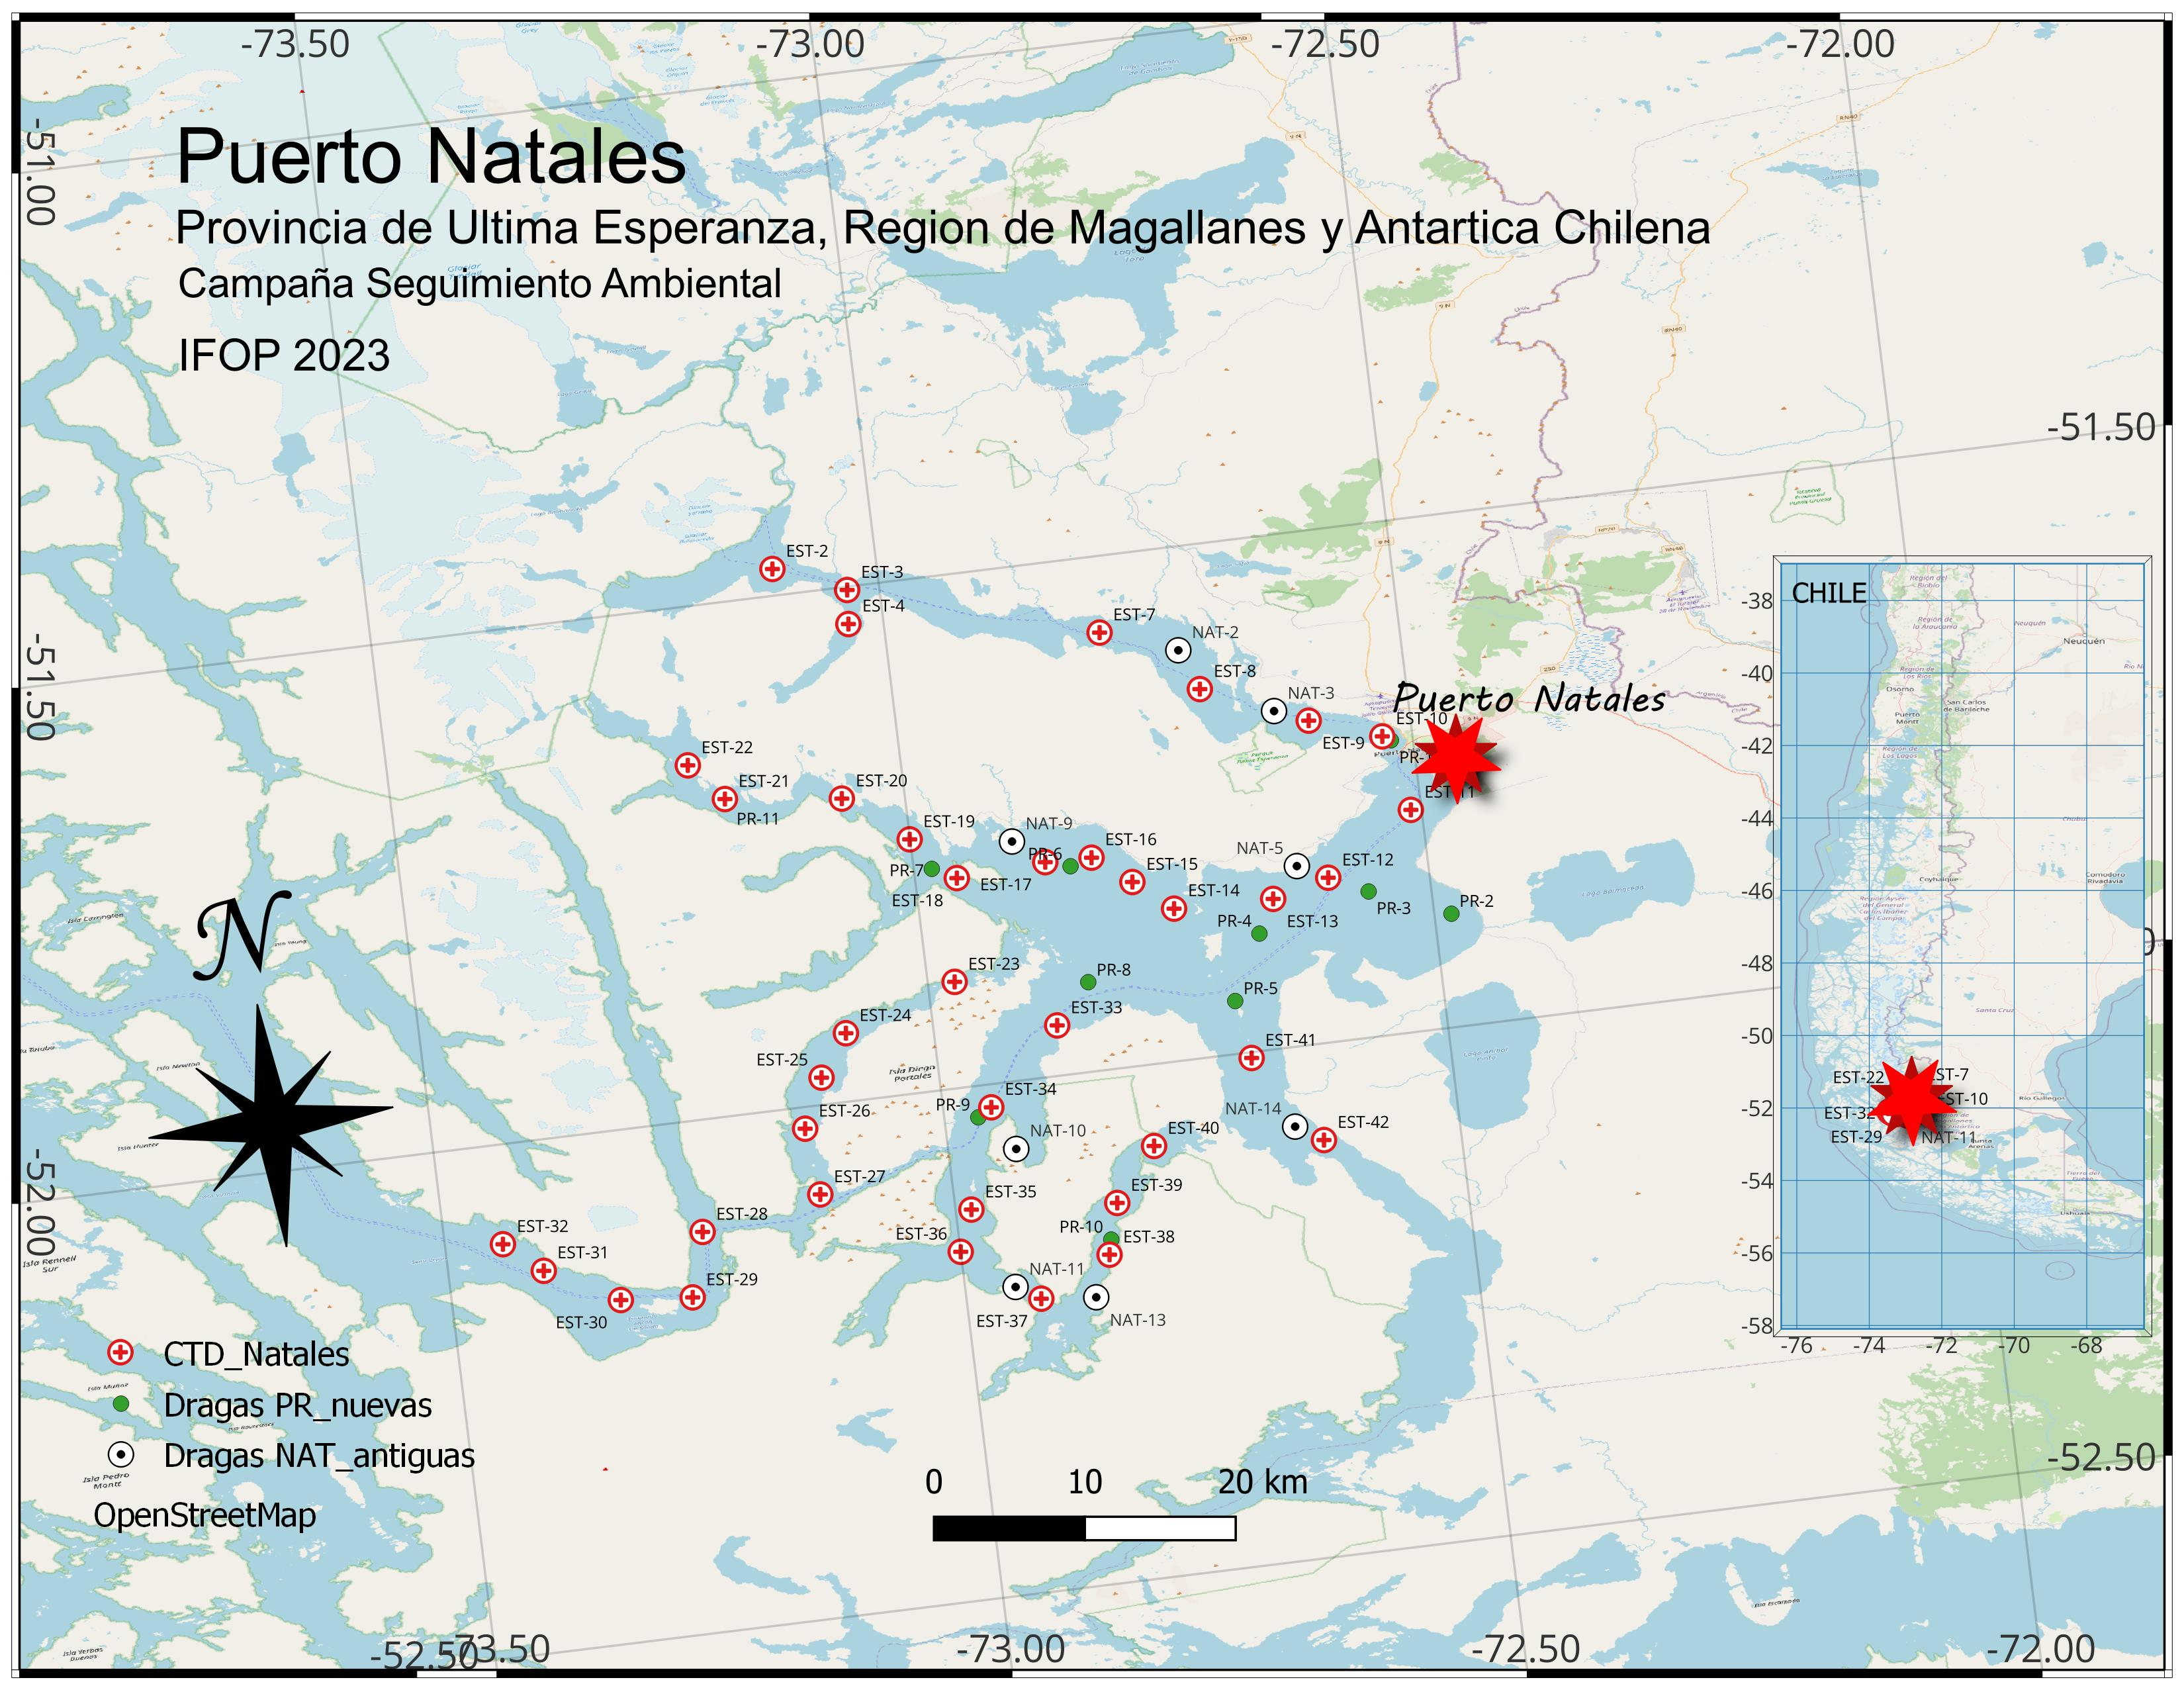
\includegraphics{images/Mapa natales_5.jpeg}

Figura 1. Mapa del crucero

\begin{figure}

{\centering 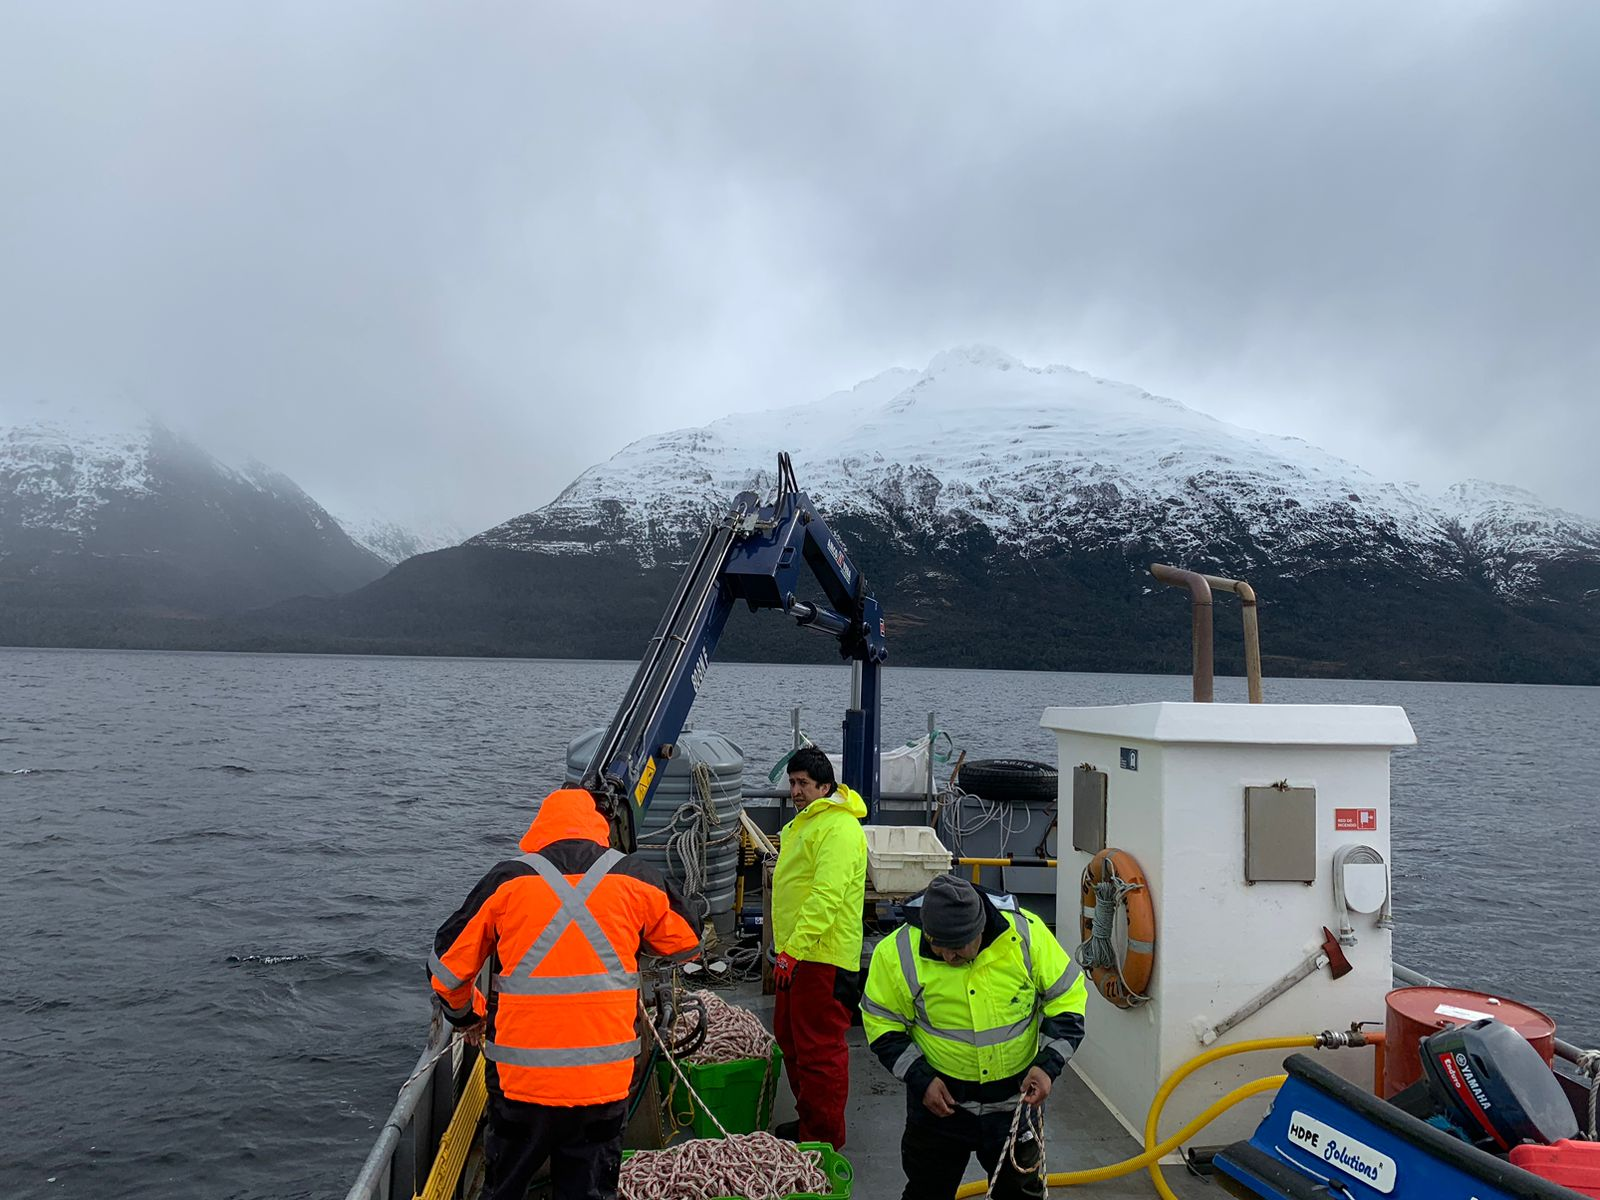
\includegraphics[width=6.84375in,height=5.84375in]{WhatsApp Image 2023-09-06 at 13.03.25.jpeg}

}

\end{figure}

Figura 2. Operaciones en cubierta

\begin{figure}

{\centering 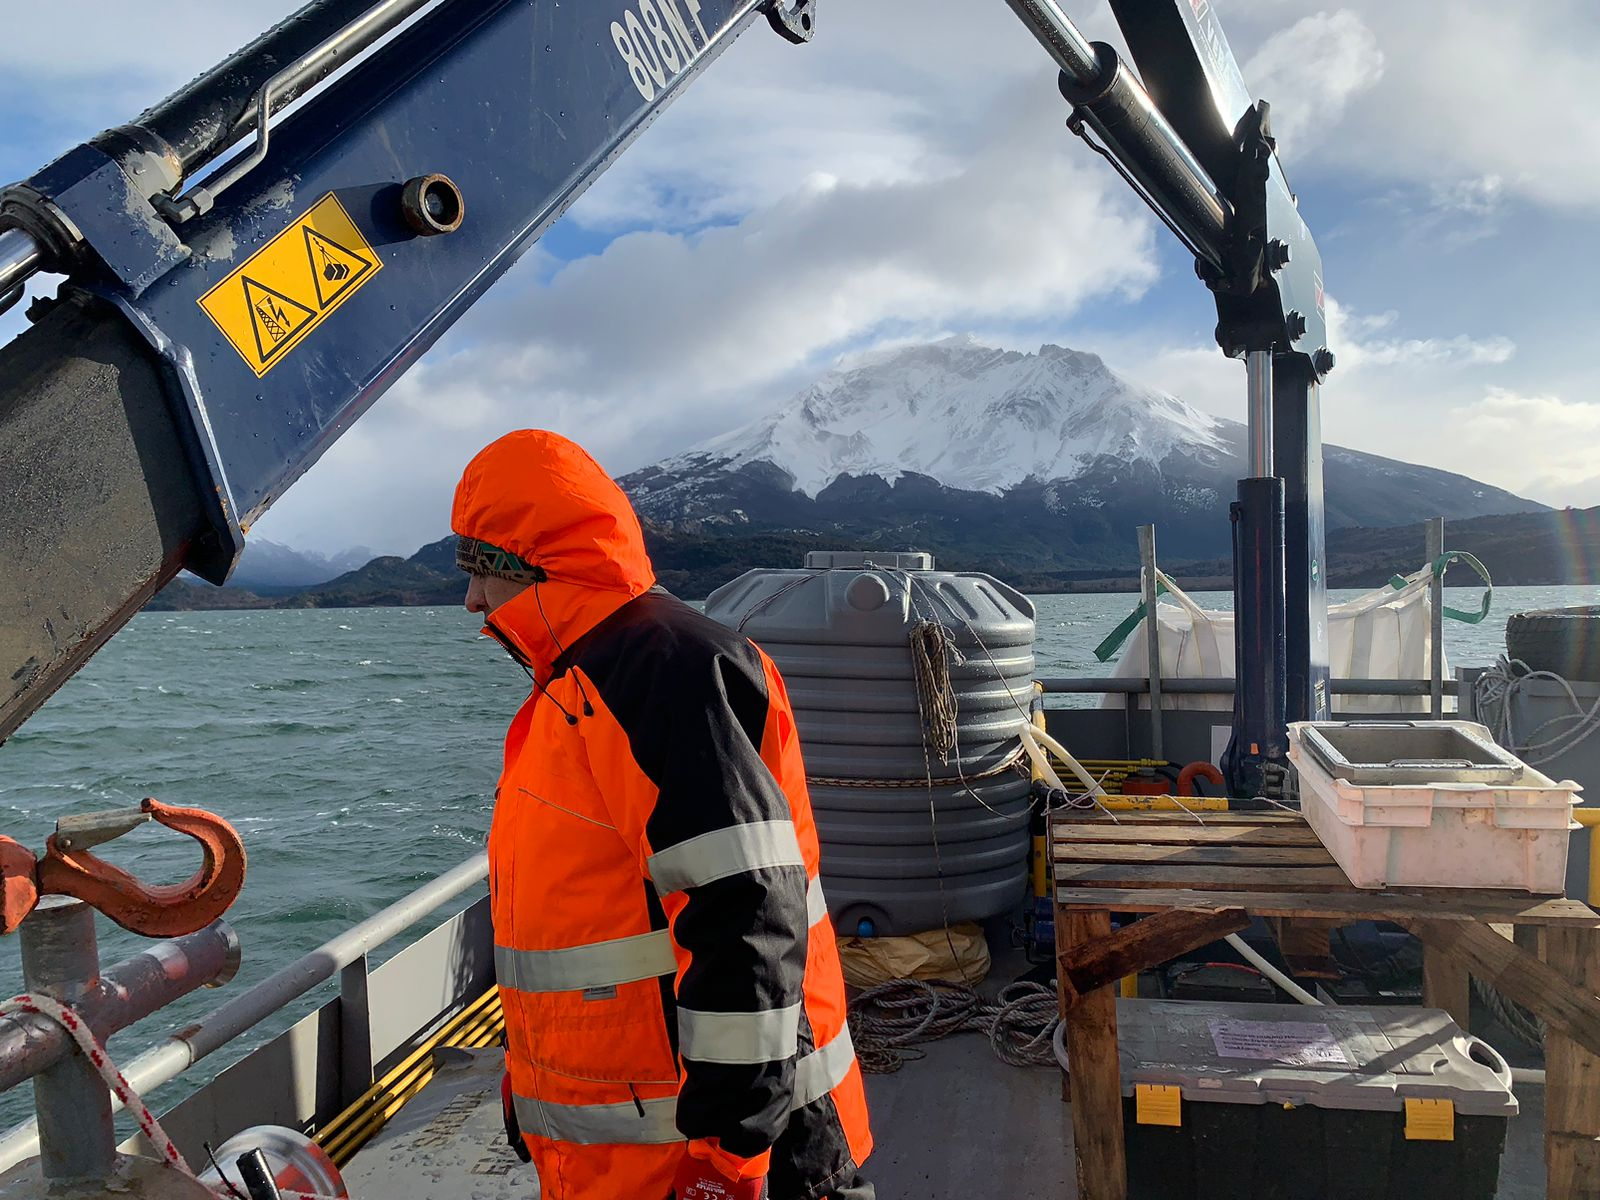
\includegraphics[width=6.69792in,height=\textheight]{WhatsApp Image 2023-09-06 at 12.41.03 (2).jpeg}

}

\end{figure}

Figura 3. Operaciones en cubierta

\begin{figure}

{\centering 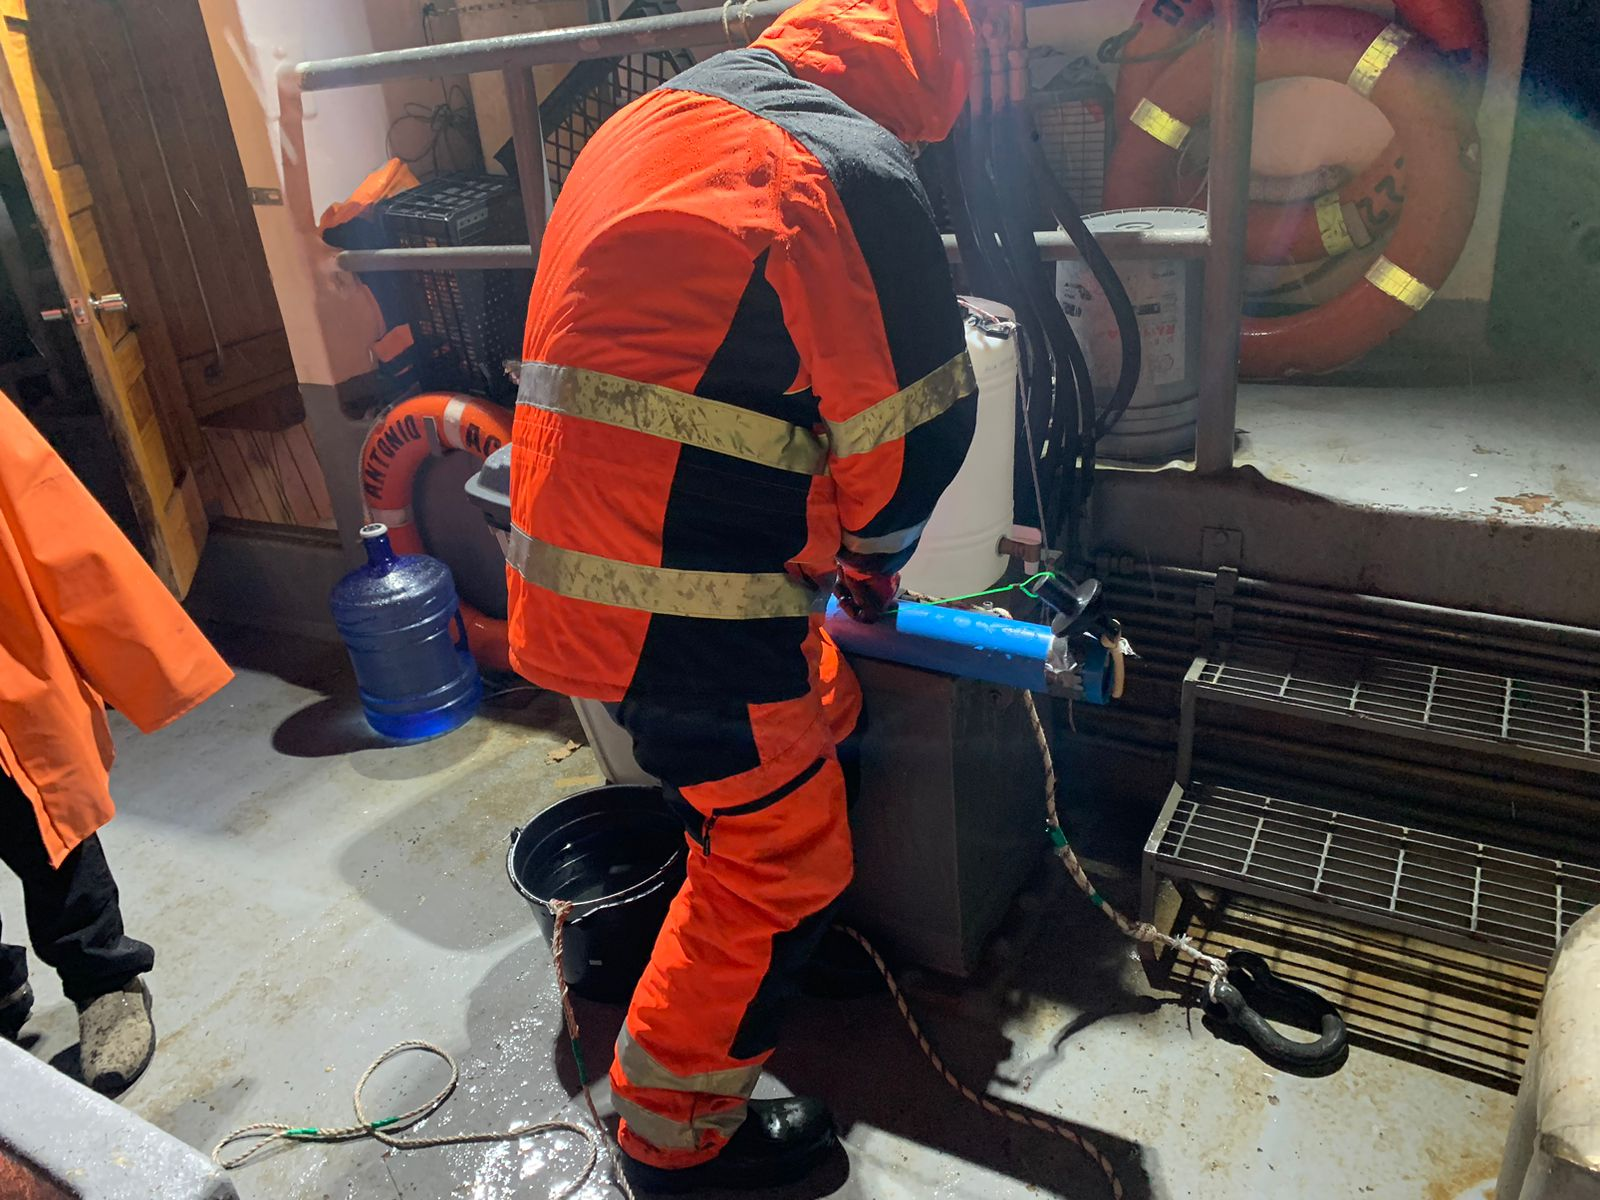
\includegraphics[width=7.04167in,height=\textheight]{WhatsApp Image 2023-09-06 at 12.41.04.jpeg}

}

\end{figure}

Figura 4. Operaciones en cubierta

\begin{figure}

{\centering 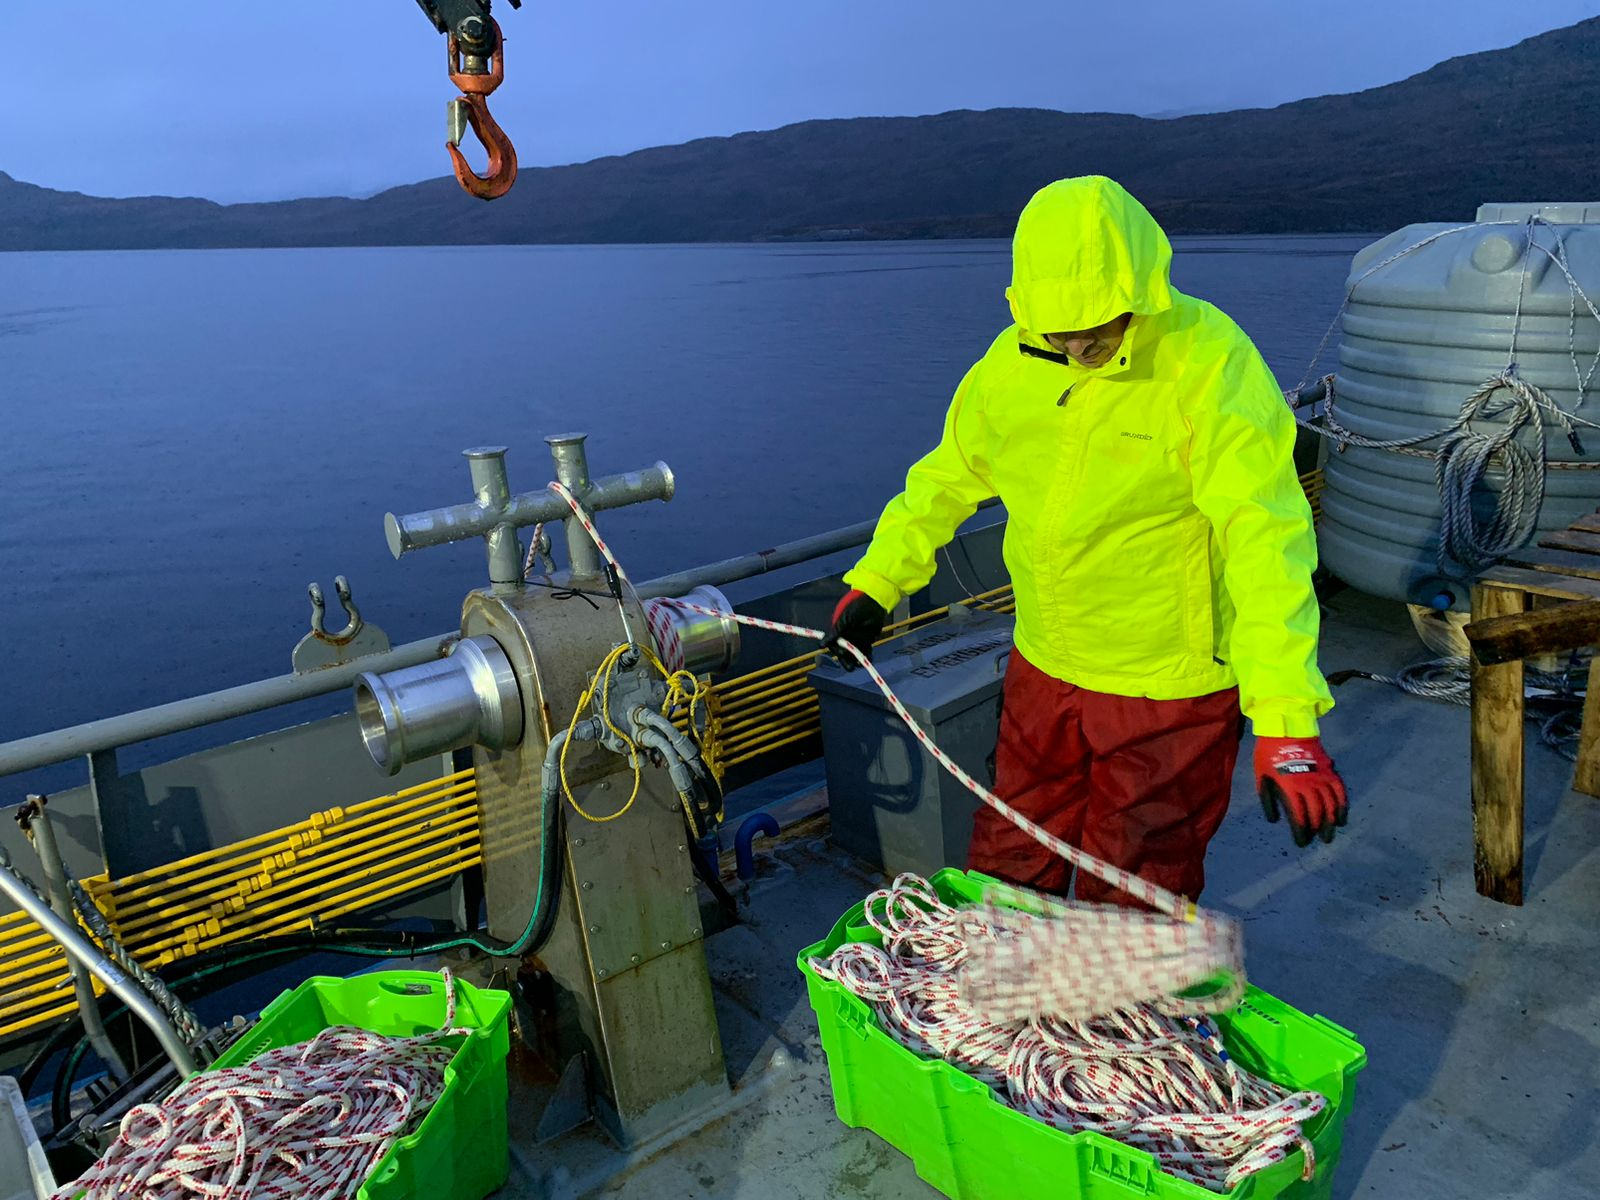
\includegraphics{WhatsApp Image 2023-09-06 at 12.41.05.jpeg}

}

\end{figure}

Figura 5. Operaciones en cubierta

\begin{figure}

{\centering 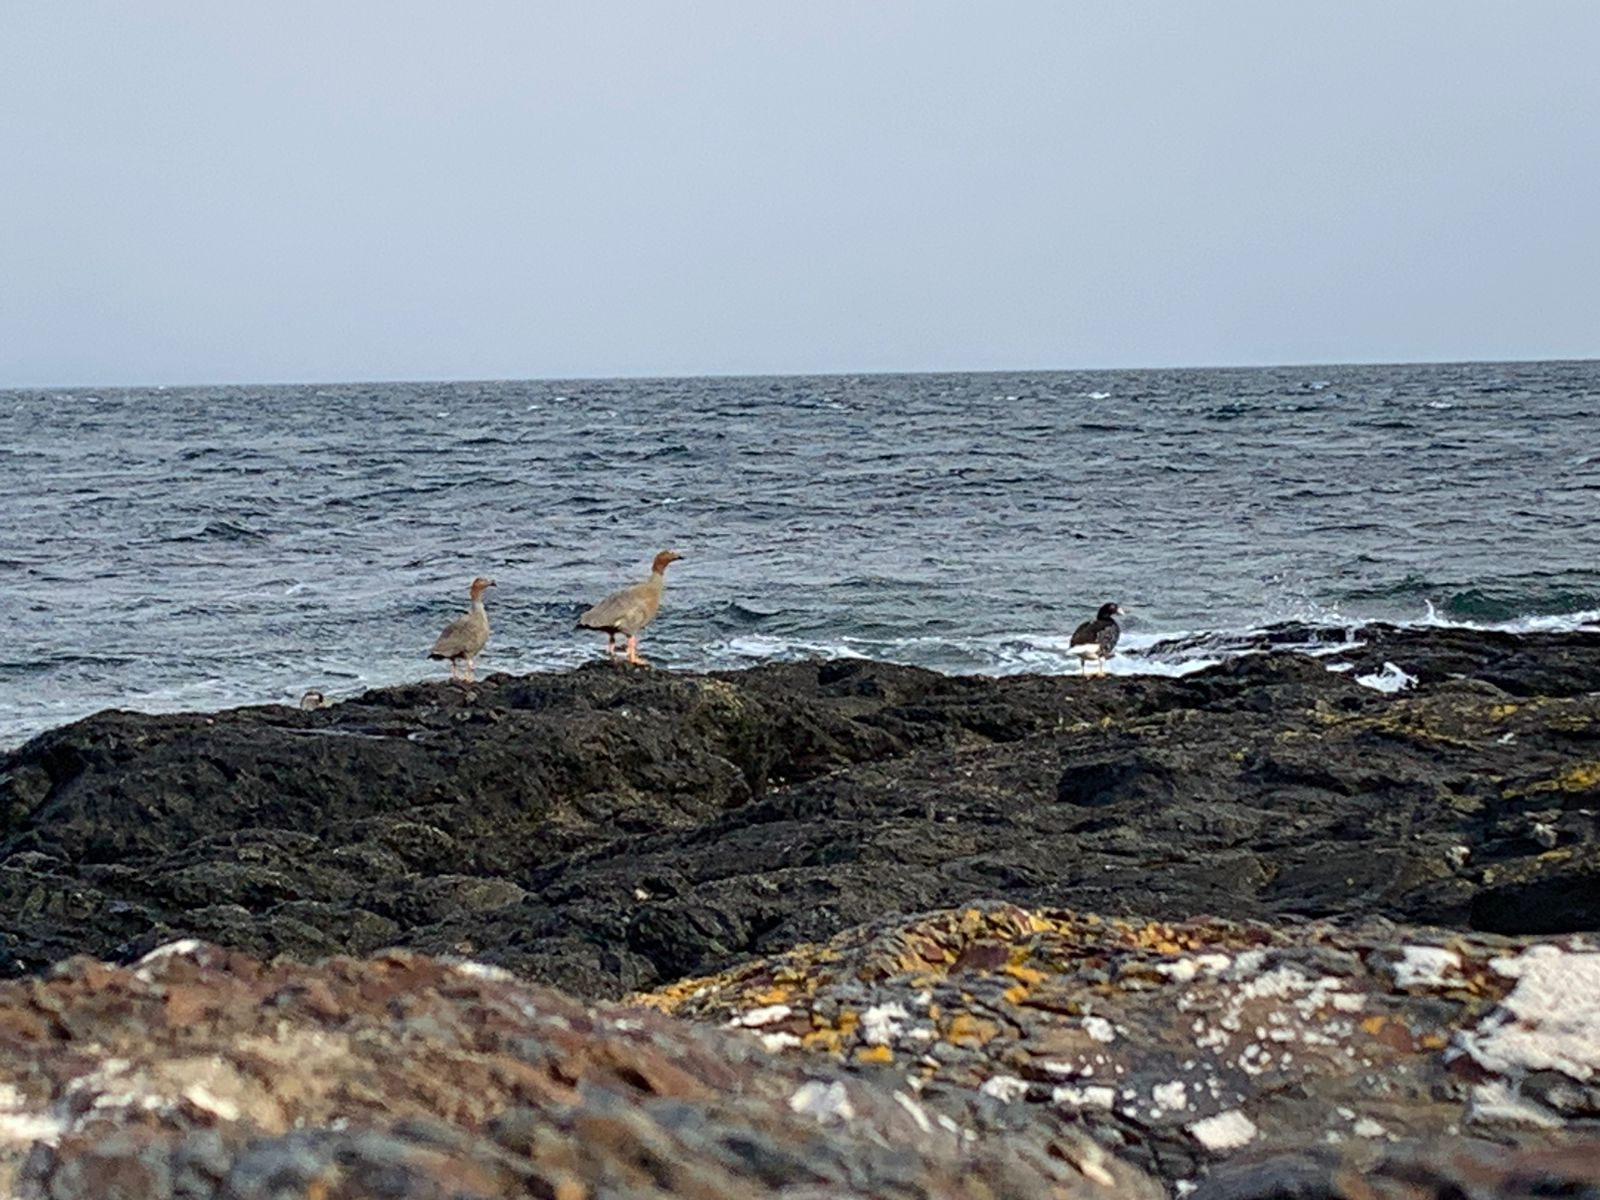
\includegraphics{WhatsApp Image 2023-09-06 at 12.41.02.jpeg}

}

\end{figure}

Figura 6. caiquenes \emph{(Chloephaga picta)} y carancas
\emph{(Chloephaga hybrida)}

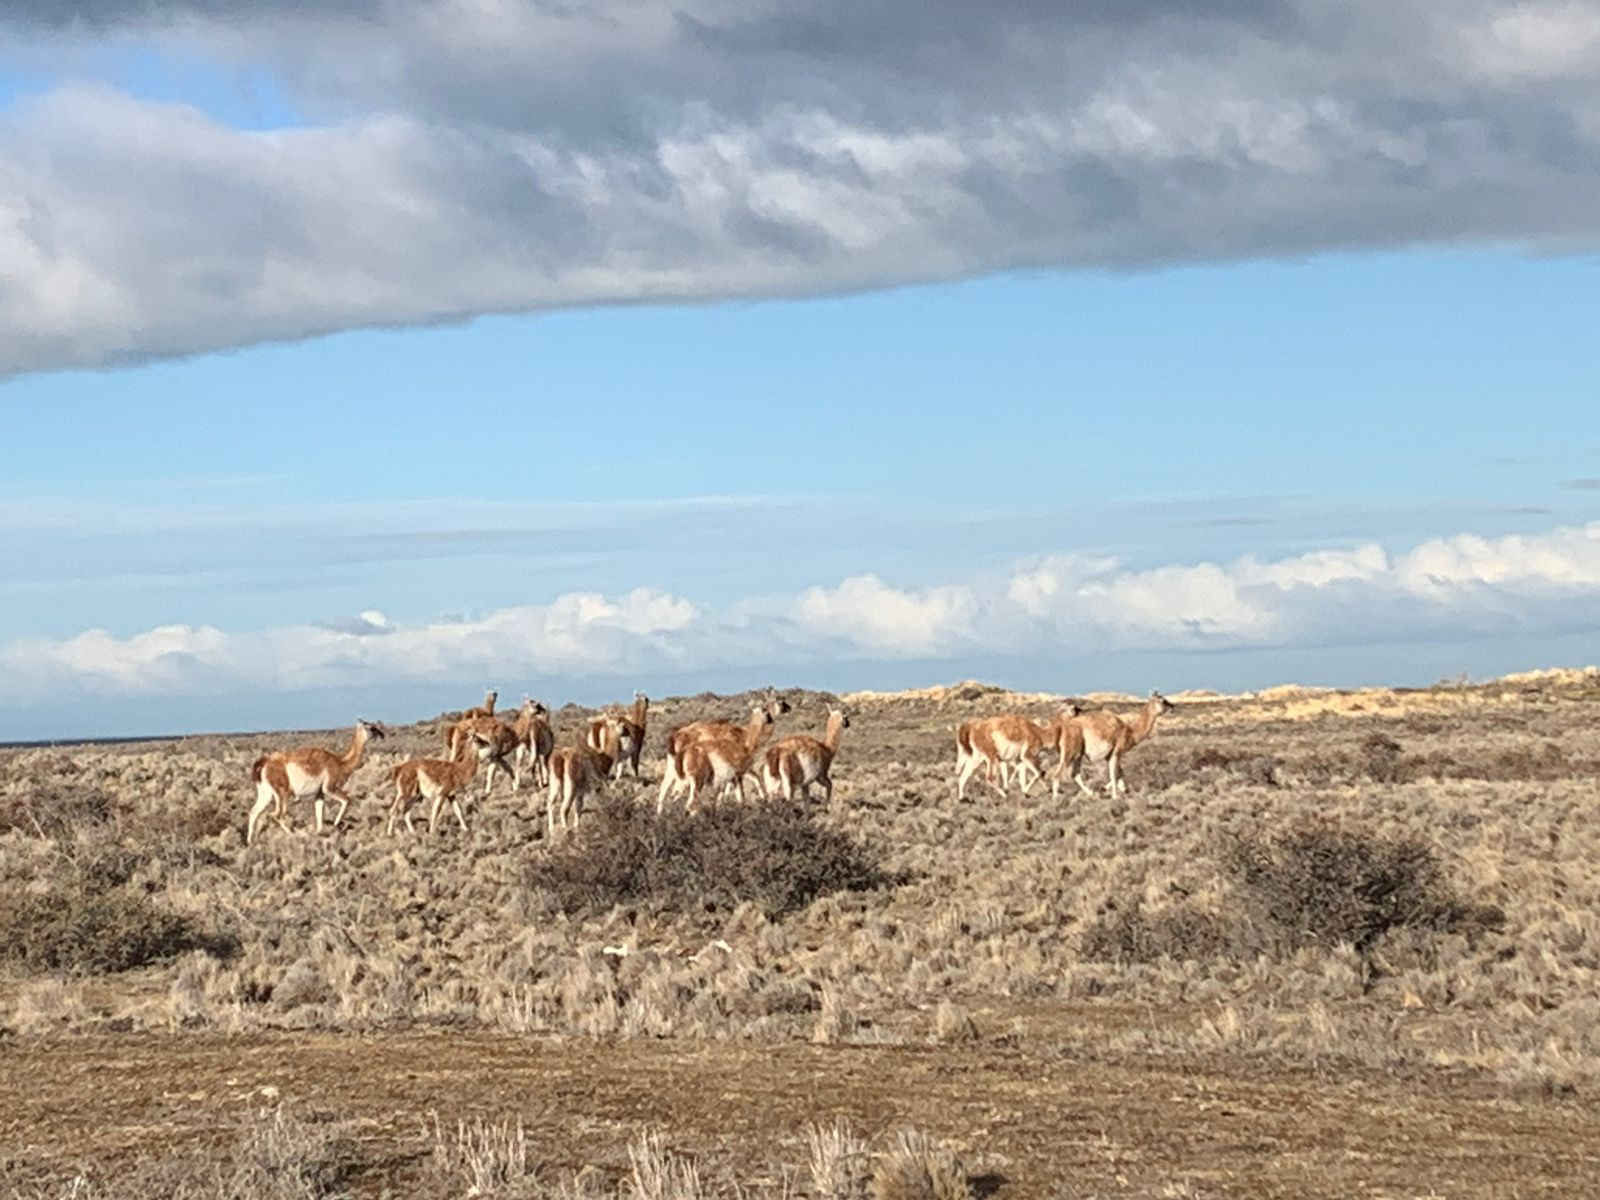
\includegraphics{WhatsApp Image 2023-09-06 at 13.06.09.jpeg}

Figura 7. Guanacos \emph{(Lama guanicoe)}

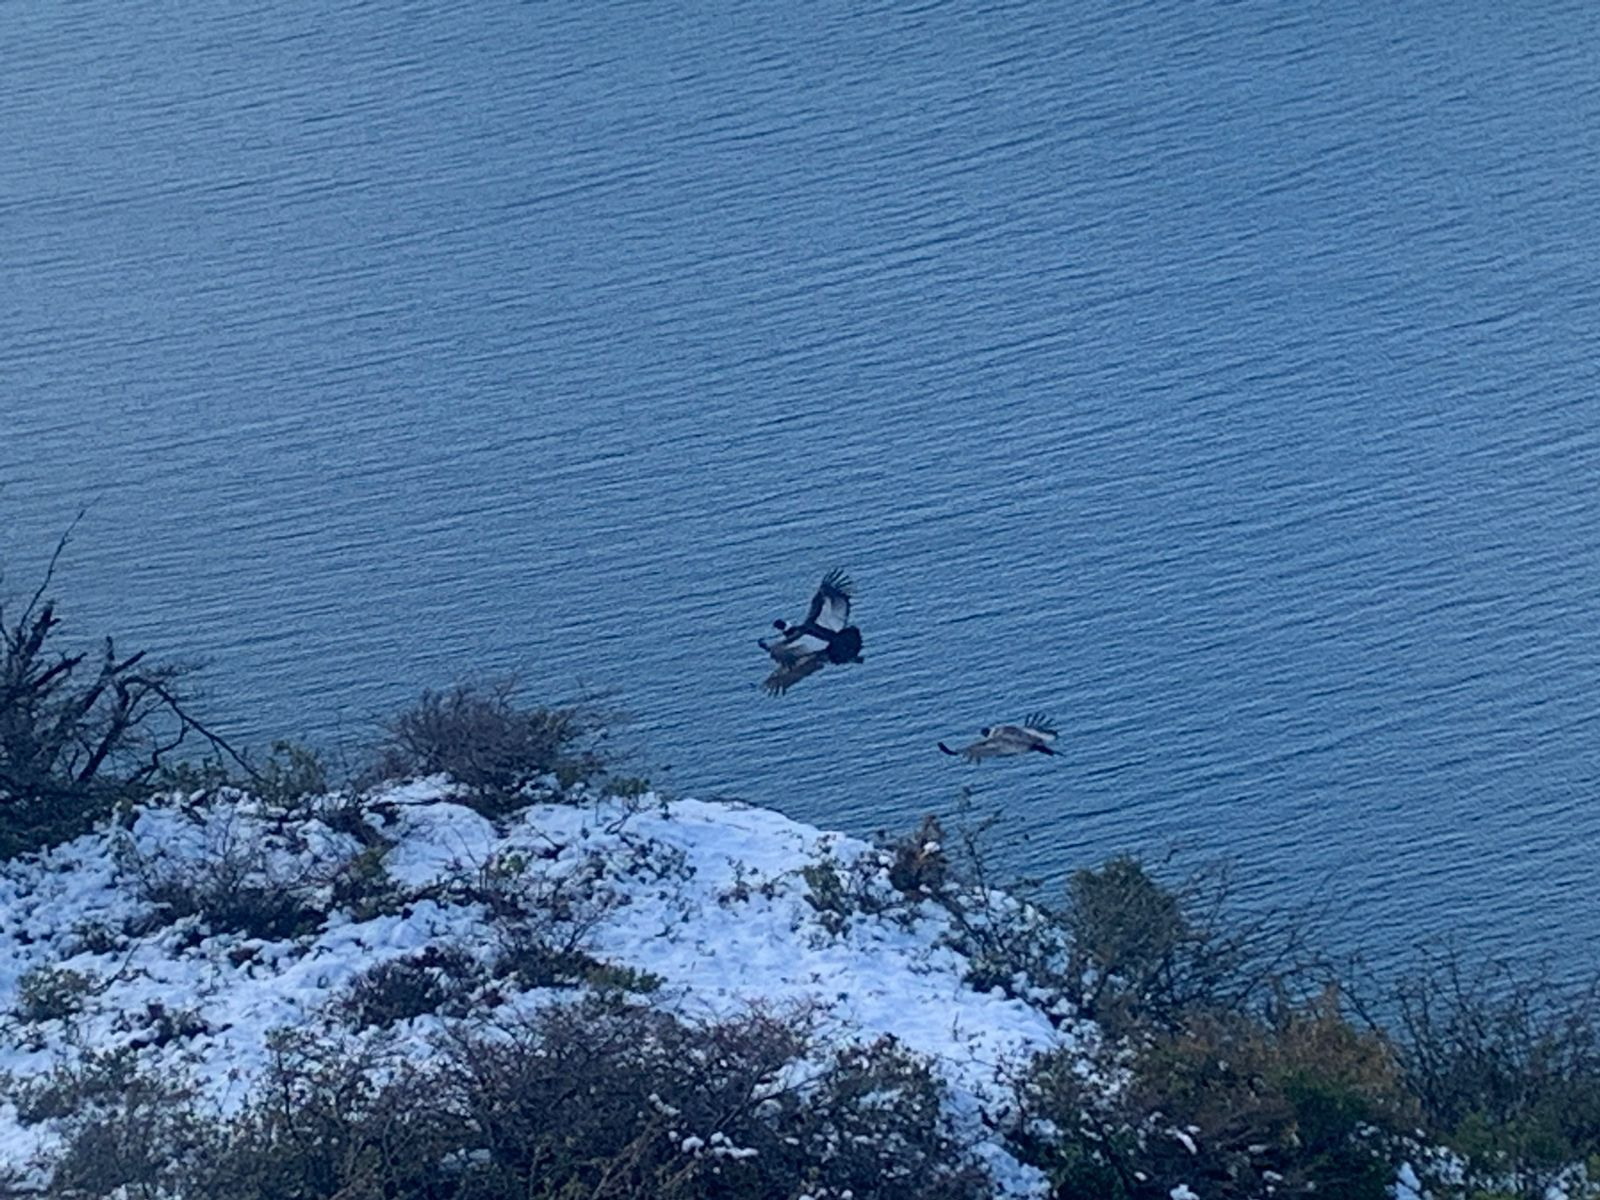
\includegraphics{WhatsApp Image 2023-09-06 at 12.58.03.jpeg}

Figura 8. condores \emph{(Vultur gryphus)}

\begin{figure}

{\centering 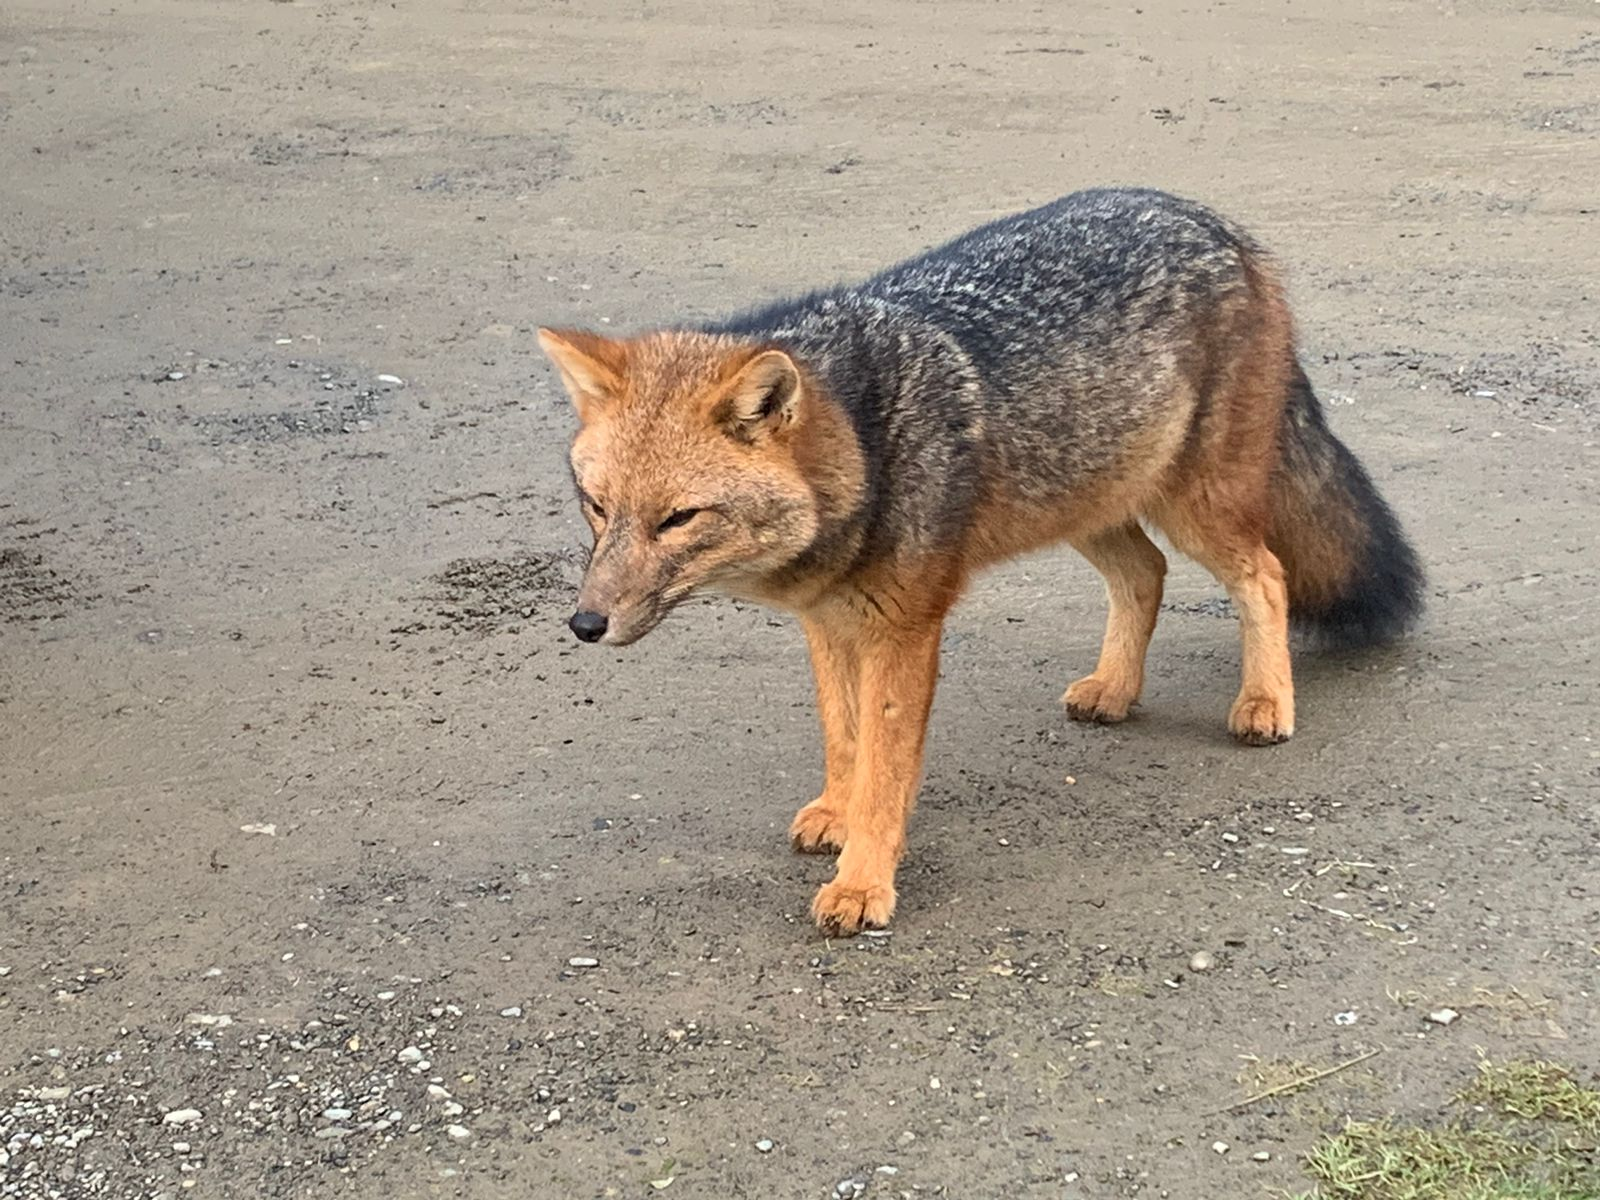
\includegraphics{WhatsApp Image 2023-09-06 at 12.41.00.jpeg}

}

\caption{Figura 9. zorros \emph{(Lycalopex culpaeus)}}

\end{figure}



\end{document}
